\section{Graph transformation with eMoflon}

The next part of our Tutorial is dedicated to the creation of a graph transformation rule set which allows us to create a concrete model instance based on constraints and multiplicities we defined in this metamodel. The goal of the ruleset we want to define in the next chapter is to achieve the defined structure and behavior of operations in our hospital while creating a certain kind of dynamic through the application of rules. This might sound a bit confusing for now, but no worries we will explain it to you step by step.

\subsection{Rules and patterns introduction}

The GitHub site where you have found this PDF for the Tutorial also has different stages of the project stored for you in case you messed something up, skipped a part of the tutorial, or if you are unsure whether everything you did is correct.
These different stages of the project are represented by different branches in the Git repository. Throughout this tutorial, we will be using four different branches which you can access to keep the project up to date for every section of the tutorial. Whenever you can switch to a new branch for a new section it will be announced at the beginning of the respective section.\newline

\textbf{Please use the branch \textsf{Ecore+GT empty} for the following section}.
This stage of the project includes the hospital ecore model and the graph transformation project you just created in the previous chapter but has some repetitive contents added to it so that you can focus on the important functionalities.\newline
Whenever you have to add code to the existing project it will be said \textbf{explicitly} and \textbf{highlighted in the Java project}.\newline

Now that you are good to go, it is time to get familiar with the two most common constructs for eMoflon Graph Transformations: \textbf{The rules and patterns}. For a more detailed description you can read the second chapter of this essay\footnote{\href{https://www.cs.le.ac.uk/people/rh122/papers/2006/Hec06Nutshell.pdf}{Graph Transformation in a Nutshell}}.\newline

\textbf{Graph pattern}:\newline
A Graph pattern describes certain structures that must be present in a given instance graph. A structure consists of an arangement of nodes with specific types and specific connecting edges. On the other hand a pattern could also be made up by a single node of a specified type.\newline
\begin{figure}[h]
    \centering
    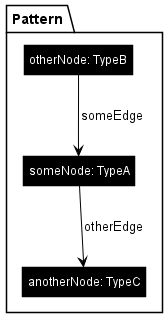
\includegraphics[scale=0.7]{pictures/pattern.png}
    \caption{\centering{Pattern example in PlantUML}}
    \label{pattern example}
\end{figure}

Consequently, a graph pattern matcher will find all sub-structures in the instance graph that match all structural constraints of a given pattern.\newline
\clearpage

\textbf{Graph transformation rule}:\newline\newline
A graph transformation rule consists of a so-called left-hand side (LHS) and right-hand side (RHS). The former describes certain preconditions, like a graph pattern, that must be present in a given instance graph, otherwise, a rule is not applicable. If a match of the LHS is found, the rule can be applied. When a rule is applied, the graph is changed in such a way, that the rule's RHS is satisfied. More precisely, any graph pattern node and edge that is present in the LHS, but is not present in the RHS, is deleted. In turn, any node that is not present in the LHS, but is present in the RHS, is created.\newline

\begin{figure}[h]
    \centering
    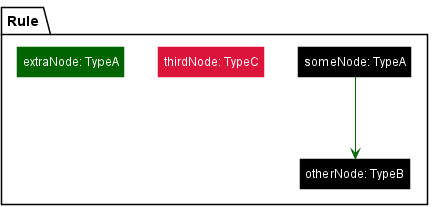
\includegraphics[scale=0.8]{pictures/rule.png}
    \caption{\centering{A rule example in PlantUML}}
    \label{rule}
\end{figure}

\clearpage

\subsection{Creating a graph transformation project}

Let us get started by creating a new eMoflon Graph Transformation project. Please click on the button \ref{item:2} with the \textbf{red and green arrow in the folder}.\newline\newline

\centering

→ Please write \textsf{"HospitalTransformRules"} as the name → Press \textsf{"Finish"} \newline\newline

\raggedright

You will notice the \textsf{Rules.gt} file which has been generated automatically. In this file, you will be defining the rules to construct our Hospital.\newline
Start with deleting the automatically generated contents in the “.gt” file except for the Ecore import.

The next thing you want to do is to \textbf{import the metamodel} you have created in the previous section. Just type import and use code completion (Ctrl+Space) to obtain the suggested URI to your metamodel HospitalExample.\newline

Afterwards your \textsf{Rules.gt} file should be empty exept these two imports:\newline

{\setstretch{1.2}

1\hspace{0.5cm}\textcolor{Purple}{import} "\textcolor{Blue}{http://www.eclipse.org/emf/2002/Ecore}"

2\hspace{0.5cm}\textcolor{Purple}{import} "\textcolor{Blue}{platform:/resource/HospitalExample/model/HospitalExample.ecore}"\newline

}

You might have noticed that the project has some \textbf{compilation errors}. To solve the issues do the following:\newline\newline

\centering

Open \textsf{"META-INF/MANIFEST.MF"} file → \textsf{dependencies} → Add \textsf{"HospitalExample"} from drop down menu.\newline\newline

\begin{figure}[h]
    \centering
    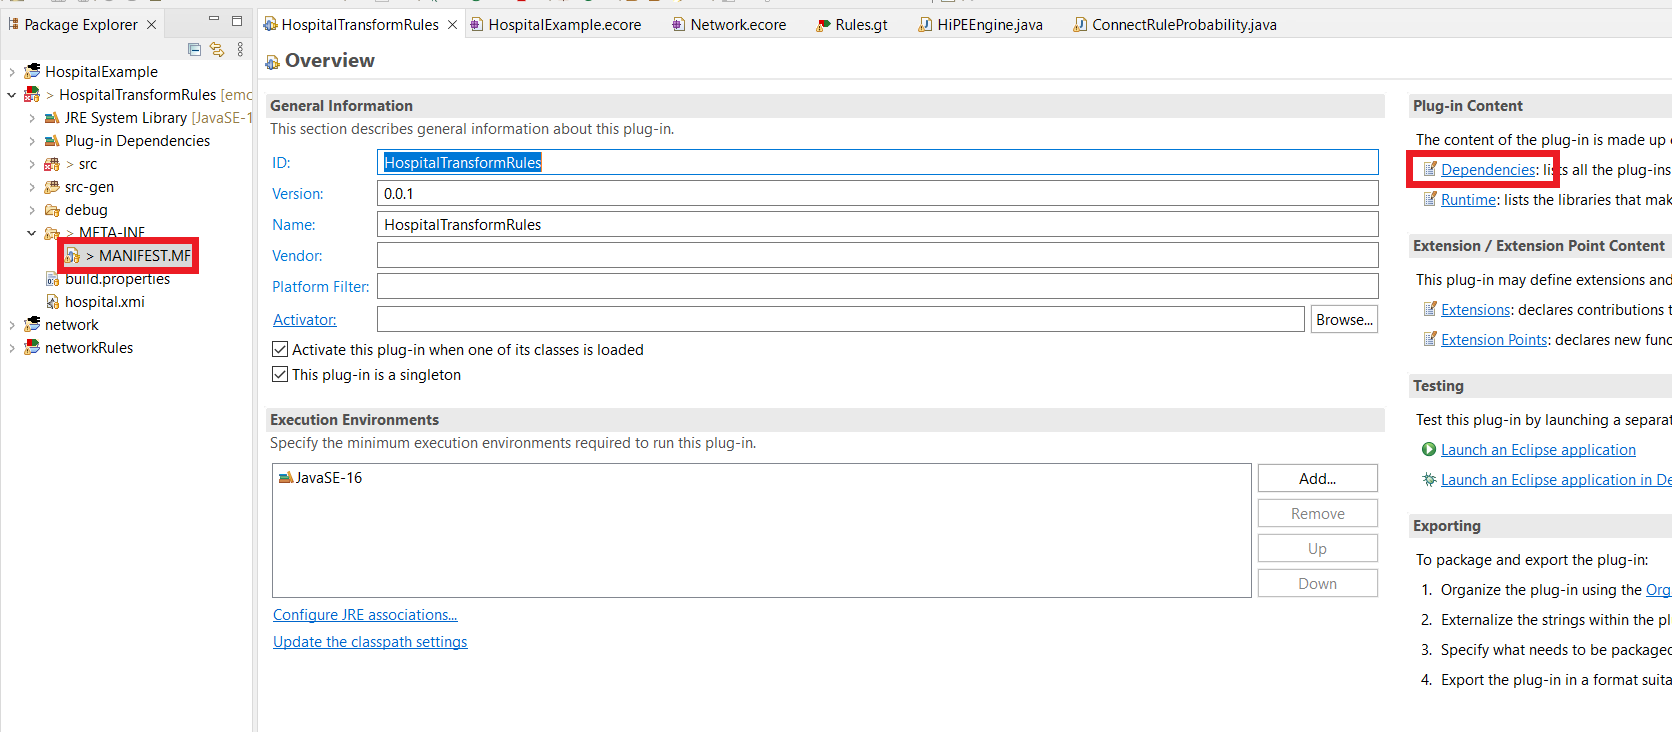
\includegraphics[scale=0.7, width= \textwidth]{pictures/manifest.png}
    \caption{\centering{Manifest.MF}}
    \label{manifest}
\end{figure}

\raggedright

The errors should be fixed now, and your project should compile properly. If the \textbf{errors persist} check if the Build automatically option is turned on in the project drop-down menu of your eclipse. \textbf{Refreshing and cleaning} all the projects are the remaining options if you are still encountering errors.

\raggedright

\clearpage
\subsection{Rules and patterns in eMoflon}

Anyhow, let us get started by writing the very first rule for our hospital rule set. The complete hospital ruleset will allow us to create a concrete hospital model instance according to the specifications of our metamodel from chapter one. Graph transformation rules are perfectly suited for this task since they allow us to consider constraints and requirements directly.\newline

\textbf{Rules:}\newline
For a rule, we need the \textbf{keyword rule} and a \textbf{name for the rule}. As previously mentioned, you should \textbf{name the rule after its purpose} to keep the project comprehensive.\newline

As a brief introduction to our syntax, we would like to present the two most important operators:

\begin{itemize}
    \item \textcolor{LimeGreen}{++} 
    \item {\color{red} -- -- }
\end{itemize}
Any Element that is prepended with a \textcolor{LimeGreen}{ ++} is \textbf{created} when the rule is applied. This is indicated by the \textcolor{LimeGreen}{ green syntax color}.\newline

In turn, the {\color{red} -- -- } operator will lead to a \textbf{deletion} of the denoted element. If an element is deleted by the application of a rule the {\color{red}syntax will be colored red}. \newline

If none of the operators is used, the element is interpreted as \textbf{context} and \textbf{colored as black}.\newline

Every element that is \textbf{not denoted} with an operator describes the \textbf{LHS} of the rule, which means that these elements must be present in a given instance graph.\newline
In practical terms, a valid match of the LHS must be present before the rule can be applied.\newline
By using the \textcolor{LimeGreen}{++} operator before the hospital graph pattern node in the hospital rule, we enable the rule to create a new hospital Object upon application. Since this rule has no black or red context elements, it can \textbf{always} be applied. \newline

{\setstretch{1.2}

1  \hspace{0.5cm}  \textcolor{Purple}{rule} hospital() \{\newline
2  \hspace{1cm}  \textcolor{LimeGreen}{++hospital: Hospital}\newline
3  \hspace{0.5cm}  \}\newline

}

\textbf{Patterns:}

If we want to check whether a hospital object is present within a given model, we can create a pattern that finds a hospital. Here we create the pattern \textsf{findHospital()} that defines a node named hospital of the type Hospital. Since no elements are annotated with any of the operators, findHospital() only contains black elements, i.e., context and will not lead to the creation or deletion of any objects.\newline
Therefore, findHospital() is not a rule, but a pattern, which solely will instruct the pattern matching engine to \textbf{find matches of this pattern}.\newline

{\setstretch{1.2}

4 \hspace{0.5cm}	{\color{Purple}pattern} findHospital() \{\newline
5 \hspace{1cm}	hospital: Hospital\newline
6 \hspace{0.5cm}	\}\newline

}

\textbf{Please create rule and pattern in the \textsf{Rules.gt} file of your \textsf{HospitalTransformRules} project.}\newline


\textbf{Note on the visualization of PlantUML}:
\newline
When you click on the freshly created hospital rule you should see the visualization in the PlantUML window on the right. It shows you the rule and the way the rule is defined as a graph structure. The black boxes are pattern nodes that represent context, as a consequence these nodes must be present in an instance graph. Analogously, black arrows define context edges between nodes, that must be present in the same instance graph. The green elements are the ones we are creating with a rule application.

\clearpage

\subsection{Application Condition}

Since our model requires only one hospital node, we should add a so-called \textbf{application condition} to prevent multiple applications of the hospital rule.\newline

A condition has to be defined and needs to be accessed by the keyword \textcolor{Purple}{when} to use it. To define a condition, you need to type \textcolor{Purple}{condition} and its \textbf{name}.

\textbf{Note:} The \textbf{condition expression} works like a variable and can be used in the context of other rules and patterns once assigned.\newline

Please note there are two types of conditions. You can either \textcolor{Purple}{forbid} the presence of graph structures attached to pattern matches or \textcolor{Purple}{enforce} them.
An application condition that forbids the presence of such structures is called a \textbf{negative application condition (NAC)} while a condition that enforces the presence of such structures is called a \textbf{positive application condition (PAC)}.
\newline
The utilization of a construct consisting of a condition and a pattern is called a \textbf{support pattern invocation} while the pattern itself is called a \textbf{support pattern}.\newline \newline
Back to the example. To extend our hospital rule with a negative application condition, add a \textcolor{Purple}{when} behind our hospital rule and insert \textsf{fordbidHospital} as the name of the condition. Now we need to specify our condition to prevent the creation of another hospital object if we already have one.\newline
With our condition, we want to forbid the application of the rule if our \textsf{findHopistal} pattern finds the structure \textsf{hospital:Hospital}.\newline

{\setstretch{1.2}

1 \hspace{0.5cm} \textcolor{Purple}{condition} forbidHospital = \textcolor{Purple}{forbid} findHospital 

2 \hspace{0.5cm} \textcolor{Purple}{rule} hospital() \{ 

3 \hspace{1cm} \textcolor{LimeGreen}{++ hospital: Hospital}

4 \hspace{0.5cm} \}

5 \hspace{0.5cm} \textcolor{Purple}{when} forbidHospital \newline


}

After creating a rule for the construction of a hospital node we need to fill our hospital with the same objects of our meta-model. So, let us continue with a \textbf{reception}. We start by creating the rule \textsf{reception} and adding a reception node of the type of reception.\newline

In contrast to the previous rule, we also have to \textbf{link our reception to the hospital}. To create such a reference, we require the hospital node and add an edge from the hospital node to the reception node as we have done previously in the tutorial.\newline You need to use the \textcolor{LimeGreen}{++} operator once again but now we continue with a \textbf{"-"}. This marks the created structure as an edge. The \textbf{“-"} is followed by the \textbf{type of the edge} and with \textbf{“->”} we are pointing towards the \textbf{node we want to connect}.\newline
The syntax should look like depicted below and the crucial part for the creation of an edge is shown in \textbf{line 8}:\newline

{\setstretch{1.2}

6 \hspace{0.5cm}\textcolor{Purple}{condition} forbidReception = \textcolor{Purple}{forbid} findReception

7 \hspace{0.5cm}\textcolor{Purple}{rule} reception() \{

8 \hspace{1cm}     hospital: Hospital \{

9 \hspace{1.5cm}       \textcolor{LimeGreen}{++ -reception -> reception}

10 \hspace{1.5cm}	 \}

11 \hspace{0.5cm}	 \textcolor{LimeGreen}{++reception: Reception}

12 \hspace{0.5cm}\}

13 \hspace{0.5cm}\textcolor{Purple}{when} forbidReception \newline

}

\textbf{Please implement both rules above this chapter in your rules file.}\newline

\clearpage

\subsection{Parameters and attribute constraints}

The focus of this chapter will be the handling of parameters in rules and attribute constraints.
Regarding the infrastructure of our hospital, we have to address the \textbf{departments} and \textbf{rooms} in our next rules.\newline

You should be able to create the \textbf{department rule and the branch} from the hospital node yourself. We will expand them now.\newline

After creating these two rules we want to introduce some new syntax. Remember that both classes have attributes that need to be assigned. To assign \textbf{attributes} you need to use the \textbf{operator “.”}. Pressing the \textbf{auto-completion} behind the "." should suggest the \textbf{attributes defined in the meta-model}.\newline By typing the \textbf{operator “:=”} you can \textbf{assign a value} to the attribute, e.g. the simplest assignment would be a static one.\newline
As an \textbf{unrelated} example for this, you could assign the \textsf{ID 1} to the department you create by writing: \newline

1 \hspace{0.5cm} .\textcolor{LimeGreen}{dID}:=\textcolor{Purple}{1}. \newline

In reality we want to hand over a \textbf{parameter}, not unlike it is done in Java methods.\newline
We need to define the parameters the rule expects in the \textbf{round brackets} after the rule name and type \textbf{param::}\textsf{paramName} instead of the static assignment. The same has to be done for \textsf{maxRoomCount}:\newline\newline

{\setstretch{1.2}

1\hspace{0.5cm} \textcolor{Purple}{rule} department(dID: EInt, maxRoomCount: EInt)\{\newline
2\hspace{1cm}	hospital: Hospital \{\newline
3\hspace{1.5cm}	\textcolor{LimeGreen}{++ -department -> department} \newline
4\hspace{1cm}	\}\newline
5\hspace{1cm}   \textcolor{LimeGreen}{++department: Department} \{ \newline
6\hspace{1.5cm}	    .\textcolor{LimeGreen}{dID}:=\textcolor{Purple}{param}::dID \newline
7\hspace{1.5cm}	    .\textcolor{LimeGreen}{maxRoomCount}:=\textcolor{Purple}{param}::maxRoomCount \newline
8\hspace{1cm}		\} \newline
9\hspace{0.5cm}\} \newline\newline

10\hspace{0.5cm} \textcolor{Purple}{rule} room(cap: EInt, carelvl: Carelevel) \{ \newline
11\hspace{1cm}		hospital: Hospital \{ \newline
12\hspace{1.5cm}			-department -> department \newline
13\hspace{1cm}		\} \newline
14\hspace{1cm}		department: Department \{ \newline
15\hspace{1.5cm}\textcolor{LimeGreen}{++ -rooms -> room} \newline
16\hspace{1cm}	\} \newline
17\hspace{1cm}	\textcolor{LimeGreen}{++room: Room} \{ \newline 
18\hspace{1.5cm}	.\textcolor{LimeGreen}{capacity}:= \textcolor{Purple}{param}::cap \newline
19\hspace{1.5cm}	.\textcolor{LimeGreen}{level}:= \textcolor{Purple}{param}::carelvl \newline
21\hspace{1cm}\} \newline
22\hspace{1cm}	\textcolor{Purple}{\#}department.maxRoomCount>\textcolor{Purple}{count}(findRoomInDepartment) \newline
23\hspace{0.5cm}\} \newline\newline

}

\textbf{Please implement both rules above this chapter in your rules file.}\newline

\clearpage

\textbf{Attribute constraints:}

For the room rule, we want to add a \textbf{constraint} that limits the creation of rooms in a certain department because we have previously limited the maximum number of rooms a department can contain. To specify a so-called \textbf{attribute constraint (or attribute condition)} you have to use the \textbf{“\#”} operator. Such an attribute constraint can be defined at any point in the pattern. For this constraint, we want to get the \textsf{maxRoomCount} of the given Department and check if the limit of rooms in this department is not exceeded.

To \textbf{access an attribute value} of a specific pattern node, we provide a syntax that is remarkably similar to accessing attributes in java, namely using the \textbf{"."} operator.\newline
For example, we access the parameter of the department node via \textsf{\#department.maxRoomCount}. The \textsf{ count(findRoomInDepartment)} instruction \textbf{counts the matches} for a certain pattern, in our case for the \textsf{findRoomInDepartment} pattern which we have to create in the next step.\newline

\textbf{Support pattern invocations with mapping:}\newline
Our goal for this pattern is to count the number of rooms which are assigned to a department. However, we want to avoid finding matching rooms connected to any department node since this would lead to \textsf{n·m} matches for \textsf{n} rooms and \textsf{m} departments.\newline Consequently, we want to count the matches for the rooms assigned to a \textbf{single} department node. In other words we want the \textbf{graph pattern matcher} to only find matches of our \textbf{pattern} \textsf{findRoomInDepartment()} that involve the \textbf{specific department node} we are currently referencing in our \textbf{rule} \textsf{room}. To accomplish this we have to create a \textbf{mapping} between the nodes in the rule and the elements in the support pattern. eMoflon will do exactly that if we \textbf{assign identical names} for the nodes in rules and patterns.\newline

Generally, patterns which are used like this, are invocated from the \textbf{'perspective'} of the currently evaluated element. eMoflon will try to resolve identifiers from the pattern as \textbf{references} to structures from the surrounding element. If matching names are found the corresponding element will be regarded as a placeholder for any node, reference or else of matching type. These kinds of pattern invocations are also called \textbf{support pattern invocations} just like \textbf{NACs} and \textbf{PACs}.\newline

You can note the difference when comparing these slightly different patterns:\newline

{\setstretch{1.2}

1\hspace{1cm}\textcolor{Purple}{pattern} findRoomsInAnyDepartment()\{  

2\hspace{1.5cm} otherdepartment:Department \{  

3\hspace{2cm} -rooms->otherroom 

4\hspace{1.5cm} \} 

5\hspace{1.5cm} otherroom: Room 

6\hspace{1cm}\}\newline 

}

When called as a support pattern \textbf{in context of the rule} \textsf{room} this will find $n \times m$ matches since it doesn't reference any structure from our rule and consequently would be valid for any rooms in any department node.\newline

\begin{figure}[h]
    \centering
    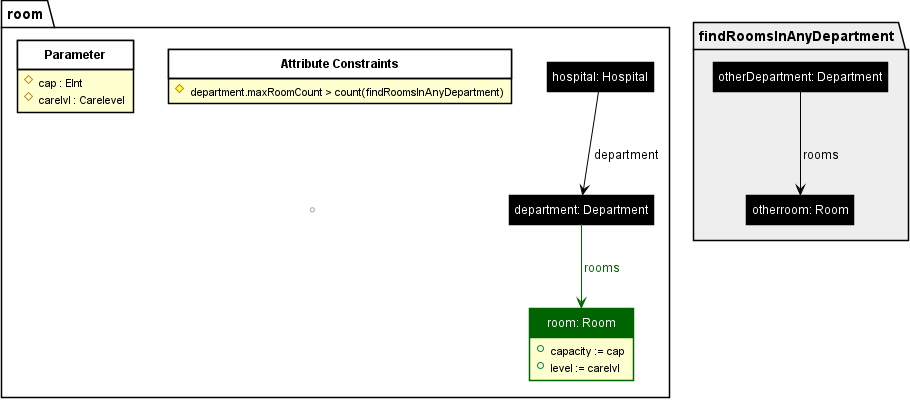
\includegraphics[scale=0.45]{pictures/findRoomsInAnyDepartment.png}
    \caption{\centering{PlantUML visualization of findRoomsInAnyDepartment}}
    \label{findRoomsAny}
\end{figure}

\clearpage


{\setstretch{1.2}

7\hspace{1cm}\textcolor{Purple}{pattern} findRoomsInDepartment()\{  

8\hspace{1.5cm} department:Department \{

9\hspace{2cm} -rooms->otherroom 

10\hspace{1.5cm} \} 

11\hspace{1.5cm} otherroom: Room 

12\hspace{1cm}\}\newline 

}

When called as a support pattern \textbf{in context of the rule} \textsf{room} this will find this pattern will find all rooms for the \textbf{specific} department node referenced in our rule.

\begin{figure}[h]
    \centering
    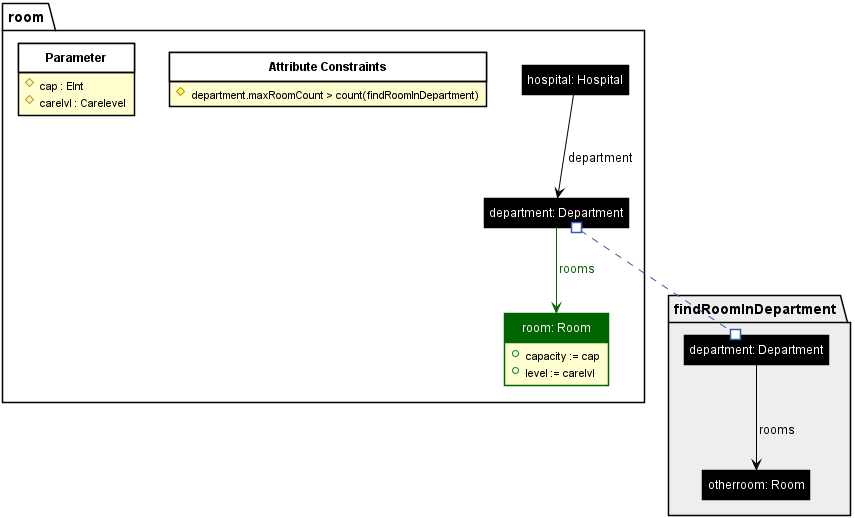
\includegraphics[scale = 0.45]{pictures/roomRule.png}
    \caption{\centering{PlantUML visualization of findRoomsInDepartment}}
    \label{findRooms}
\end{figure}

{\setstretch{1.2}

14\hspace{1cm}\textcolor{Purple}{pattern} findRoomInDepartment()\{  

15\hspace{1.5cm} department:Department \{ 

16\hspace{2cm} -rooms->room 

17\hspace{1.5cm} \} 

18\hspace{1.5cm} room: Room

19\hspace{1cm}\}\newline

}

When called like the others this pattern will find exactly find 1 match. Because we are not only referencing the department node from our rule but the specific room we have just created as well.

\begin{figure}[h]
    \centering
    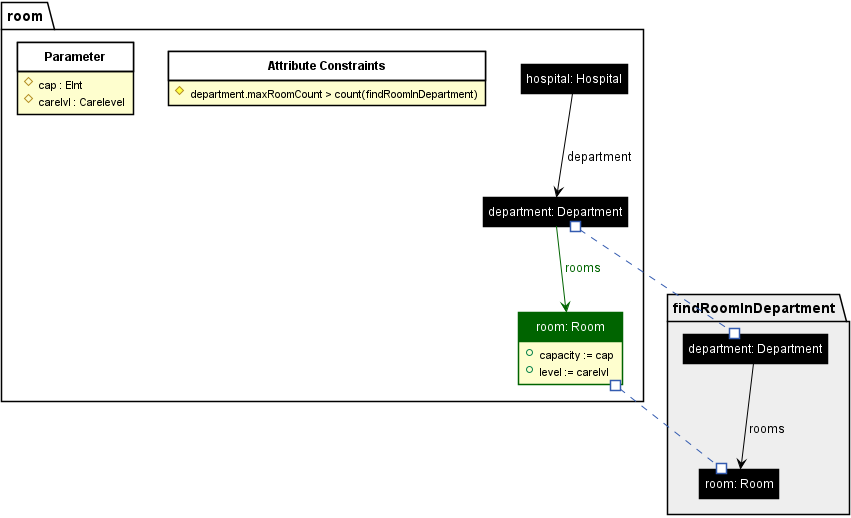
\includegraphics[scale = 0.43]{pictures/findRoomInDepartment.png}
    \caption{\centering{PlantUML visualization of findRoomInDepartment}}
    \label{attributeConstrains}

\end{figure}

Note that you can look at the PlantUML visualization of rules and pattern by clicking on them in the \textsf{rules.gt} and looking the PlantUML view. \newline

Please use the \textsf{findRoomsInDepartment} pattern for our room rule.\newline

\textbf{Disclamer control flow:}\newline
While attribute constraints and conditions can be used to model complex application conditions for rules and patterns
it's not possible to model \textbf{control flow} directly in eMoflon. For example you can not specify on which of all fitting elements a rule will be applied or in what order new elements will be created.

This has to be done in the actual code implementation.



\clearpage

\subsection{Finishing the graph transformation ruleset}

After we have created the ruleset for the infrastructure of the hospital, we need rules to define the behavior of the persons in the hospital. In our case, we have the following person types in our hospital: the \textbf{patients}, the \textbf{doctors}, and the \textbf{nurses}.\newline

\textbf{Patients:}\newline
For the patients, we assume that a patient appears in the reception and waits there until he has been assigned to a room. Naturally, a patient has a name, an age and will be assigned a patientID and carelevel which requires a certain kind of treatment.\newline\newline

{\setstretch{1.2}

1\hspace{0.5cm}\textcolor{Purple}{rule} patient(name: EString,age: EInt, patientId: EInt, level: Carelevel) \{

2\hspace{1cm}	hospital: Hospital \{

3\hspace{1.5cm}	-reception -> reception 

4\hspace{1cm}	\}

5\hspace{1cm}	reception: Reception \{

6\hspace{1.5cm}	\textcolor{LimeGreen}{++ -waits -> patient }

7\hspace{1cm} \}

8\hspace{1cm}	\textcolor{LimeGreen}{++patient: Patient} \{

9\hspace{1.5cm} .\textcolor{LimeGreen}{name}:=\textcolor{Purple}{param}::name

10\hspace{1.5cm}.\textcolor{LimeGreen}{patientID}:=\textcolor{Purple}{param}::patientId

11\hspace{1.5cm}.\textcolor{LimeGreen}{level}:=\textcolor{Purple}{param}::level

12\hspace{1.5cm}.\textcolor{LimeGreen}{age}:=\textcolor{Purple}{param}::age

13\hspace{1cm} \}

14\hspace{0.5cm} \} \newline\newline

}

Another important use case that one can think of is the dismissal of a patient, which can be modeled with a the following rule.\newline For this rule, we want to \textbf{remove} a patient with a given \textsf{patientID} by using the \textbf{operator} \textcolor{red}{-- --}.\newline
To keep our model clean, we also want to \textbf{avoid dangling edges}. The EMF framework removes those dangling edges automatically, but we can also remove the edges manually.
An example for the edges we remove in the rule \textsf{releasePatient} would be in \textbf{lines 84 and 87}.\newline\newline

{\setstretch{1.2}

80\hspace{0.5cm}\textcolor{Purple}{rule} releasePatient(patientID:EInt)\{

81\hspace{1cm}\textcolor{red}{-- -- patient: Patient}\{

82\hspace{1cm}\}

83\hspace{1cm}room: Room\{

84\hspace{1.5cm}\textcolor{red}{-- -- -lies -> patient}

85\hspace{1cm}\}

86\hspace{1cm}doctor: Doctor\{

87\hspace{1.5cm}\textcolor{red}{-- -- -caresfor -> patient}

88\hspace{1cm}\}

89\hspace{1cm}\textcolor{Purple}{\#}patient.patientID==\textcolor{Purple}{param}::patientID

90\hspace{0.5cm}\}\newline\newline

}

\clearpage

\textbf{Staff:}\newline
According to our metamodel, the class Staff is \textbf{abstract}. Every staff member is assigned to a department and has a name and a staffID as parameters to identify staff members. \newline
A note on abstract rules: Just like it is not possible to instantiate an abstract class in Java it is \textbf{not possible to apply an abstract rule}. However, elements such as nodes, edges, and parameters will be inherited by a refining rule.\newline\newline

{\setstretch{1.2}

15\hspace{0.5cm}\textcolor{Purple}{abstract rule} staff(name: EString, staffID: EInt) \{ 

16\hspace{1cm}		hospital: Hospital \{

17\hspace{1.5cm}\textcolor{LimeGreen}{++ -staff -> staff} 

18\hspace{1.5cm}			-department -> department

19\hspace{1cm}		\}

20\hspace{1cm}		department : Department

23\hspace{1cm}\textcolor{LimeGreen}{++staff: Staff} \{ 

24\hspace{1.5cm}		.\textcolor{LimeGreen}{staffID}:=\textcolor{Purple}{param}::staffID

25\hspace{1.5cm}			.\textcolor{LimeGreen}{name}:=\textcolor{Purple}{param}::name

26\hspace{1cm}		\}

27\hspace{0.5cm}	\}\newline\newline

}


\textbf{Doctors:}\newline
Since the doctor rule is a specification of the staff rule, we can \textbf{refine} this rule to save some writing effort and improve readability. This can be done by adding the \textbf{keyword} \textsf{refines} and the rule which should be refined to the head of your rule.\newline
To make things more interesting we could add another condition to our doctor rule. The condition only assigns a doctor to a department if the given department has no doctor who is already responsible for the department. Hence, we need a fitting pattern in addition to our doctor’s rule.\newline
This pattern works analogously to the pattern we defined for the rooms.\newline\newline

{\setstretch{1.2}

29\hspace{0.5cm}\textcolor{Purple}{condition} departmentWithoutDoctor  = \textcolor{Purple}{forbid} doctorInDepartment 

30\hspace{0.5cm}\textcolor{Purple}{rule} doctor(capacity: EInt) \textcolor{Purple}{refines} staff \{ 

31\hspace{1cm}\textcolor{LimeGreen}{++staff: Doctor} \{

32\hspace{1.5cm}.\textcolor{LimeGreen}{patientCapacity}:=param::capacity

33\hspace{1cm}\}

34\hspace{1cm}		department : Department \{

35\hspace{1.5cm}\textcolor{LimeGreen}{++ -staff -> staff}

36\hspace{1cm}\}

37\hspace{0.5cm}\}

38\hspace{0.5cm}\textcolor{Purple}{when} departmentWithoutDoctor \newline

41\hspace{0.5cm}\textcolor{Purple}{pattern} doctorInDepartment() \{

42\hspace{1cm}		someDoctor : Doctor

43\hspace{1cm}		department : Department \{

44\hspace{1.5cm}			-staff -> someDoctor

45\hspace{1cm}  \}

46\hspace{0.5cm}\}\newline\newline

}
\clearpage

\textbf{Nurse:}\newline
eMoflon is capable of distinguishing between the two different types of staff members. Hence, we can name the nodes for both types of staff. \newline
For the nurse rule, we want to combine the creation of a nurse node with the assignment to a room. This assignment requires the creation of an edge to a room, as well as the creation of a staff node of the type nurse and a staff edge to the departments.\newline In our case, we want to assign only one nurse per room, which requires another condition and a pattern to find nurses who are already assigned to a room.\newline\newline

{\setstretch{1.2}

 

44\hspace{0.5cm}\textcolor{Purple}{condition} forbidNurse = \textcolor{Purple}{forbid} findNurseInRoom 

45\hspace{0.5cm}\textcolor{Purple}{rule} assignNurseToRoom() \textcolor{Purple}{refines} staff \{ 

46\hspace{1cm}\textcolor{LimeGreen}{++ staff: Nurse} \{

47\hspace{1.5cm}\textcolor{LimeGreen}{++ -responsible -> room}

48\hspace{1cm}\}

49\hspace{1cm}room: Room

50\hspace{1cm}department : Department \{

51\hspace{1.5cm}-rooms -> room

52\hspace{1.5cm}\textcolor{LimeGreen}{++ -staff -> staff}

53\hspace{1cm}\}

54\hspace{0.5cm}\}

55\hspace{0.5cm}\textcolor{Purple}{when} forbidNurse\newline 

62\hspace{0.5cm}\textcolor{Purple}{pattern} findNurseInRoom() \{ 

63\hspace{1cm}somenurse: Nurse \{

64\hspace{1.5cm}-responsible -> room

65\hspace{1cm}\}

66\hspace{1cm}room: Room \{

67\hspace{1cm}\}

68\hspace{0.5cm}\} \newline\newline

}

\textbf{Patterns with conditions:}\newline
Conditions can also combined with patterns to allow more complex matching criteria.

This can be useful if we are trying to find out if there is a room that has no responsible nurse:\newline

{\setstretch{1.2}

69\hspace{0.5cm}\textcolor{Purple}{condition} roomHasNoNurse = \textcolor{Purple}{forbid} findNurseInRoom

70 \hspace{0.5cm}\textcolor{Purple}{pattern} findRoomWithoutNurse()\{  

71\hspace{1cm} room: Room

72\hspace{0.5cm}\}

73\hspace{0.5cm}\textcolor{Purple}{when} roomHasNoNurse\newline\newline

}


\clearpage

To finish our hospital ruleset, we need one last rule which assigns the patients to their rooms. This rule will be the most complex so far and there is a lot we need to take into account.\newline
First, we want to assign the patient to a room by \textbf{adding} a \textsf{lies} edge to a room and \textbf{remove} the \textsf{waits} edge from the reception.\newline
But we have to keep in mind that we can only assign a patient to a room if the \textbf{room is not full}, and we want to assign a patient to a doctor, which is also only possible if the \textbf{patient limit} of the doctor is \textbf{not exceeded}. Hence, we need \textbf{two attribute constraints} for our patient rule and a \textbf{condition} that forbids the assignment to room if the patient already has a doctor.\newline\newline

{\setstretch{1.2}

91\hspace{0.5cm}\textcolor{Purple}{condition} patientWithDoc = \textcolor{Purple}{forbid} findPatientWithDoc

92\hspace{0.5cm}\textcolor{Purple}{rule} assignPatientToRoom() \{

93\hspace{1cm}patient: Patient \{

94\hspace{1cm}\}

95\hspace{1cm}room: Room \{

96\hspace{1.5cm}\textcolor{LimeGreen}{++ -lies -> patient}

97\hspace{1cm}\}

98\hspace{1cm}\textcolor{Purple}{\#}room.capacity>\textcolor{Purple}{count}(findPatientInRoom)

99\hspace{1cm}doctor: Doctor \{

100\hspace{1.5cm}\textcolor{LimeGreen}{++-caresfor -> patient}

101\hspace{1cm}\}

102\hspace{1cm}\textcolor{Purple}{\#}doctor.patientCapacity>\textcolor{Purple}{count}(findOccupiedDoc)

103\hspace{1cm}hospital: Hospital \{

104\hspace{1.5cm}-reception -> reception

105\hspace{1.5cm}-department -> department

106\hspace{1cm}\}

107\hspace{1cm}department: Department \{

108\hspace{1.5cm}-rooms -> room

109\hspace{1cm}\}

110\hspace{1cm}reception: Reception \{

111\hspace{1.5cm}\textcolor{red}{-- -- -waits -> patient}

112\hspace{1cm}\}

113\hspace{0.5cm}\}

114\hspace{0.5cm}\textcolor{Purple}{when} patientWithDoc\newline

115\hspace{0.5cm}\textcolor{Purple}{condition} docWithPatient = \textcolor{Purple}{enforce} findPatientWithDoc

116\hspace{0.5cm}\textcolor{Purple}{pattern} findPatientWithDoc() \{

117\hspace{1cm}somedoctor: Doctor \{

118\hspace{1.5cm}-caresfor -> patient

119\hspace{1cm}\}

120\hspace{1cm}patient: Patient \{

121\hspace{1cm}\}

122\hspace{0.5cm}\}\newline

124	\hspace{0.5cm}\textcolor{Purple}{pattern} findDocWithPatient() \{

125	\hspace{1cm}	somedoctor : Doctor

126	\hspace{0.5cm}\}

127\hspace{0.5cm} \textcolor{Purple}{when} docWithPatient \newline\newline

}

\textbf{Please implement all rules and patterns of this chapter in your Rules file.}\newline

\subsection{Java implementation of the ruleset}

So far, we have only written the rules without applying them. This will be our next task.

To understand how we implement our graph transformation ruleset we should take a look at the creation of a new model instance. For this step, open the \textsf{HospitalValidator.java} in the \textsf{HospitalTransformRules package}, please.\newline

The HospitalValidator file creates an empty Model with the URI \textsf{"hospital.xmi"}:\newline\newline

{\setstretch{1.2}

1\hspace{0.5cm}\textcolor{Purple}{public class} HospitalValidator \textcolor{Purple}{extends} HospitalTransformRulesHiPEApp  \{

2\hspace{1cm}\textcolor{Purple}{public} HospitalValidator() \{

3\hspace{1.5cm}createModel(URI.createURI(\textcolor{blue}{"hospital.xmi"}));

4\hspace{1cm}\}	

5\hspace{0.5cm}\}\newline

}

We use this simple class to initialize a new model instance with the name \textsf{hospital.xmi}.\newline
Let us inspect HospitalRules.java a bit more closely since there is much of interest going on:\newline\newline 

{\setstretch{1.2}

1\hspace{0.5cm}\textcolor{Purple}{public class} HospitalRules \{

2\hspace{0.5cm}…	

3\hspace{1cm}\textcolor{Purple}{private} Random \textcolor{blue}{rnd};

4\hspace{1cm}\textcolor{Purple}{public} HospitalTransformRulesAPI \textcolor{blue}{api};

5\hspace{1cm}\textcolor{Purple}{public} HospitalRules(\textcolor{Purple}{final long} \textcolor{Tan}{rndSeed}) \{

6\hspace{1.5cm}\textcolor{blue}{rnd} = \textcolor{Purple}{new} Random(\textcolor{Tan}{rndSeed});

7\hspace{1.5cm}\textcolor{blue}{api} = \textcolor{Purple}{new} HospitalValidator().initAPI();

8\hspace{1cm}\}

9\hspace{1cm}\textcolor{Purple}{public static void} main(String[] \textcolor{Tan}{args}) \textcolor{Purple}{throws} IOException \{

10\hspace{1.5cm}HospitalRules \textcolor{Tan}{hospitalrules} = \textcolor{Purple}{new} HospitalRules(\textcolor{blue}{"someSeed"}.hashCode());

11\hspace{1.5cm}\textcolor{Tan}{hospitalrules}.createHospital();

12\hspace{1.5cm}\textcolor{Tan}{hospitalrules}.validateHospital();

13\hspace{1cm}\textcolor{Purple}{try} \{

14\hspace{1.5cm}\textcolor{Tan}{hospitalrules}.\textcolor{blue}{api}.getModel().getResources().get(0).save(null); 

15\hspace{1cm}\}

16\hspace{1cm}\textcolor{Purple}{catch} (IOException e) \{

17\hspace{1.5cm}// TODO Auto-generated catch block

18\hspace{1.5cm}\textcolor{Tan}{e}.printStackTrace();

19\hspace{1cm}\}

20\hspace{1cm}\textcolor{Tan}{hospitalrules}.\textcolor{blue}{api}.terminate();

21\hspace{0.5cm}\}

22\hspace{0.5cm}\textcolor{Purple}{public void} createHospital() \{

23\hspace{1cm}\textcolor{blue}{api}.hospital().apply();

24\hspace{1cm}\textcolor{blue}{api}.reception().apply();

25\hspace{1cm}\textcolor{Purple}{for}(\textcolor{Purple}{int} \textcolor{Tan}{i}=0; \textcolor{Tan}{i}<4; \textcolor{Tan}{i}++) \{

26\hspace{1.5cm}\textcolor{blue}{api}.department(i+2, 4).apply();

27\hspace{1cm}\}

28\hspace{1cm}\textcolor{Purple}{for}(\textcolor{Purple}{int} \textcolor{Tan}{i}=0; \textcolor{Tan}{i}<16; \textcolor{Tan}{i}++) \{

29\hspace{1.5cm}\textcolor{blue}{api}.room(4, Carelevel.get(\textcolor{blue}{rnd}.nextInt(3))).apply();

30\hspace{1cm}\} 

\hspace{0.7cm}…

\hspace{0.7cm}\}

}

\clearpage

\textbf{Initialization:}

The first important thing we want to look at is in \textbf{line 4} where we define and initialize the \textbf{api variable} for our hospital transformation rules.\newline
The API command is used to access and apply our rules and patterns.\newline

\textbf{Saving the project:}

Another important thing to note is happening on \textbf{line 14} where we save our hospital model. It is important to note that the hospital instance we have initialized in the \textsf{HospitalValidator} will \textbf{not be stored} anywhere. If we want to keep it for usage in the future, we have to \textbf{save it with a separate command} as we are doing it in line 14.\newline The URI \textsf{hospital.xmi} is saved in the project folder of the \textsf{HospitalTransformRules} project.\newline

\textbf{Rule application:}

Let us take a closer look at the \textsf{createHospital} method starting at \textbf{line 22}.\newline
As you can see we are accessing our rules via the variable name \textbf{api.<rulename>.apply()}.\newline Then we construct our hospital subsequently by applying all the rules necessary for our hospital.\newline

The application of the hospital rule in \textbf{line 28} creates \textbf{one hospital object} according to our rule. Keep in mind we can only apply rules and not patterns. As previously mentioned we can access the eMoflon:IBeX functionalities via the \textbf{.api command}.\newline

Writing \textsf{.api} and pressing the hotkeys for auto-completion will show you the extensive list of commands we can use for our graph transformation project. In the appendix for this part of the tutorial, you can find a list with a short explanation of the respective command.\newline

Be aware that a rule can only be applied if the precondition is met, i.e., matches to its left-hand side exist.\newline
For example, if we switch the application order of the hospital and reception rule, we would not be able to create a reception because we are missing the context of the hospital node and the corresponding connection.\newline
Here is a faulty example if you changed the order of the rule application:\newline

\textcolor{red}{api.reception().apply();}\newline
\textcolor{red}{api.hospital().apply();}\newline

This order would have \textbf{severe consequences} for our hospital since the rules which require a reception such as the patients would not be applied as well as the reception itself. \newline

With rule applications below the reception rule, we will create persons of the type of patient, doctor, and nurse for our hospital as well as the departments and the rooms for our hospital.\newline

\textbf{Printing results:}

A basic way to check whether our rule applications had the desired effect is, to display relevant match counts on the console, using the \textsf{System.out.println(…)} \textbf{method}. This is what we are doing in the \textsf{validateHospital()} \textbf{method} where we count the matches we can find for a given pattern and print them to the console.\newline

{\setstretch{1.2}

\textcolor{Purple}{long} countPatientsInHospital = \textcolor{blue}{api}.findPatient().countMatches();

System.\textcolor{blue}{out}.println(\textcolor{Tan}{countPatientsInHospital} + \textcolor{blue}{" Patients are in the hospital right now"});\newline\newline

}

\clearpage

\textbf{Testing:}

You can run the java application by \textbf{right-clicking} on the \textsf{HospitalRule.java} and selecting the \textsf{Run as Java Application} option. If you look at the output in the console, and it should look like this:\newline

{\setstretch{1.2}

\textsf{10 Patients are in the hospital right now}

\textsf{10 Patients are in a room}

\textsf{One instance of a hospital has been created}

\textsf{At least one department instance has been created}

\textsf{16 nurses are in the hospital right now and 16 nurses are busy}

\textsf{At least one doctor is in the hospital}

\textsf{4 doctors are in the hospital right now and 4 doctors are busy}

\textsf{At least one patient is in the hospital}

\textsf{The hospital consists of at least one room}

\textsf{10 Patients are in the hospital right now and 10 patients are in a room}\newline

}

If you get a console output like this one without any errors your Java code is most likely correct, but this does not guarantee that the model instance we have created is the one you intended to create.\newline
For example, if some rules could not have been applied it would not be presented as a compilation error. Carefully examining the output for the validation of our hospital is the key to find misconceptions in our ruleset.

\clearpage

\subsection{Stochastic extension}

Now we are going to introduce rule conditions that are also dependent on \textbf{probabilities}.
The probability of a rule can be written in two ways:\newline With an arithmetic expression as or with a stochastic function. We will explore both possibilities in the following chapters.\newline
Please note, only rules can have a probability since patterns are always \textbf{deterministic}.

The probability is written at the end of the rule after a \textsf{@} . That means even if the corresponding condition is met the rule will only be applied with a chance of \textsf{probability}.
\newline

A simple example of a rule with a constant probability could be written as below:\newline

{\setstretch{1.2}

1\hspace{0.5cm}\textcolor{Purple}{rule} releasePatient(patientID:EInt)\{

\hspace{0.75cm}...

2\hspace{0.5cm} \}

3\hspace{0.5cm}\textcolor{Purple}{when} patientIsThreated @ 0.3 

4\hspace{0.5cm}\textcolor{Purple}{condition} patientIsTreated = \textcolor{Purple}{enforce}  findPatientInRoom \newline
}

The probability of this rule is now saved in a \textsf{StaticProbability} \textbf{class}, which itself is saved in the generated connect rule class.\newline

When using the stochastic extension in eMoflon it is necessary to apply the rule with \textsf{.applyStochastic()} or \textsf{.applyStochastic(M match)}. Otherwise when using the functions \textsf{.apply()} or \textsf{.apply(M match)} the rule will be applied \textbf{deterministically}.

When using \textsf{applyStochastic} it will return the corresponding match of the rule with the defined probability and \textsf{optional.empty()} else.

\subsection{Arithmetic Extension}

eMoflon also supports a lot of mathematical calculations in the form of arithmetic expressions.

They are very useful when assigning attribute values or defining attribute constrains that involve some sort of calculation.\newline

The arithmetic extension allows a variety of arithmetic functions which are depicted in the table below. With these functions, it is possible to write all sorts of equations.

eMoflon will automatically check if given input parameters are within domains of definitions for specific functions. If not an error will be displayed.\newline

Here is a list of supported operations, their respective domains of definition are of course equal to their mathematical counterparts:

\begin{itemize}
    \item Basic operators +, -, *, /, \%
    
    \item Exponents
    
    \item Exponential function
    \item Logarithmic functions
    \item Trigonometric functions cosinus, sinus, tangens
    \item Absolute value function
\end{itemize}

You can find the corresponding syntax in the \textbf{appendix}.\newline

\subsection{Static Probabilities}

Of course we want to model much more complex probabilities than a introduced in section 4.8.
One way to define probabilities is with the mentioned \textbf{arithmetic expressions}.

As an example for the former we will create a rule that is very similar to the \textsf{releasePatient} rule we have already seen. But this time we don't want to release a patient based on his ID. Instead we want to model the probability of a treatment being effective for a random patient:\newline

{\setstretch{1.2}

79\hspace{0.5cm}\textcolor{Purple}{condition} patientIsTreated = \textcolor{Purple}{enforce} findPatientInRoom 

80\hspace{0.5cm}\textcolor{Purple}{rule} releasePatientWhenHealed()\{

81\hspace{1cm}\textcolor{red}{-- -- patient: Patient}\{

82\hspace{1cm}\}

83\hspace{1cm}room: Room\{

84\hspace{1.5cm}\textcolor{red}{-- -- -lies -> patient}

85\hspace{1cm}\}

86\hspace{1cm}doctor: Doctor\{

87\hspace{1.5cm}\textcolor{red}{-- -- -caresfor -> patient}

88\hspace{1cm}\}

89\hspace{0.5cm}\}

90\hspace{0.5cm}\textcolor{Purple}{when} patientIsTreated @ (1 - \textcolor{Purple}{exp} (-\textcolor{Grey}{0.001} * (patient.age - \textcolor{Grey}{18}) $\wedge$ \textcolor{Grey}{2}))\newline

}
Note: We are using \textbf{node mapping} in this when statement to access the \textsf{age} value of the same patient node referenced in the rule.\newline

Naturally young adults have the best immune system while old people and very young children need more time to recover. We can model the corresponding chance of healing with the expression:

\centering

 $$ P(Healing) =   1 - e^{ - \frac{(age - 18)^{2}}{1000}} $$
 
 \raggedright

The actual calculations for our parameterized condition are done in a specifically generated class named \textsf{ReleasePatientWhenHealedRuleProbability}
Generally, all probabilities that are dependent on a parameter will generate a class. If there is no dependency like in the previous chapter, then the \textsf{StaticProbabilityclass} will be used for the probability calculation.\newline

\begin{figure}[h]
    \centering
    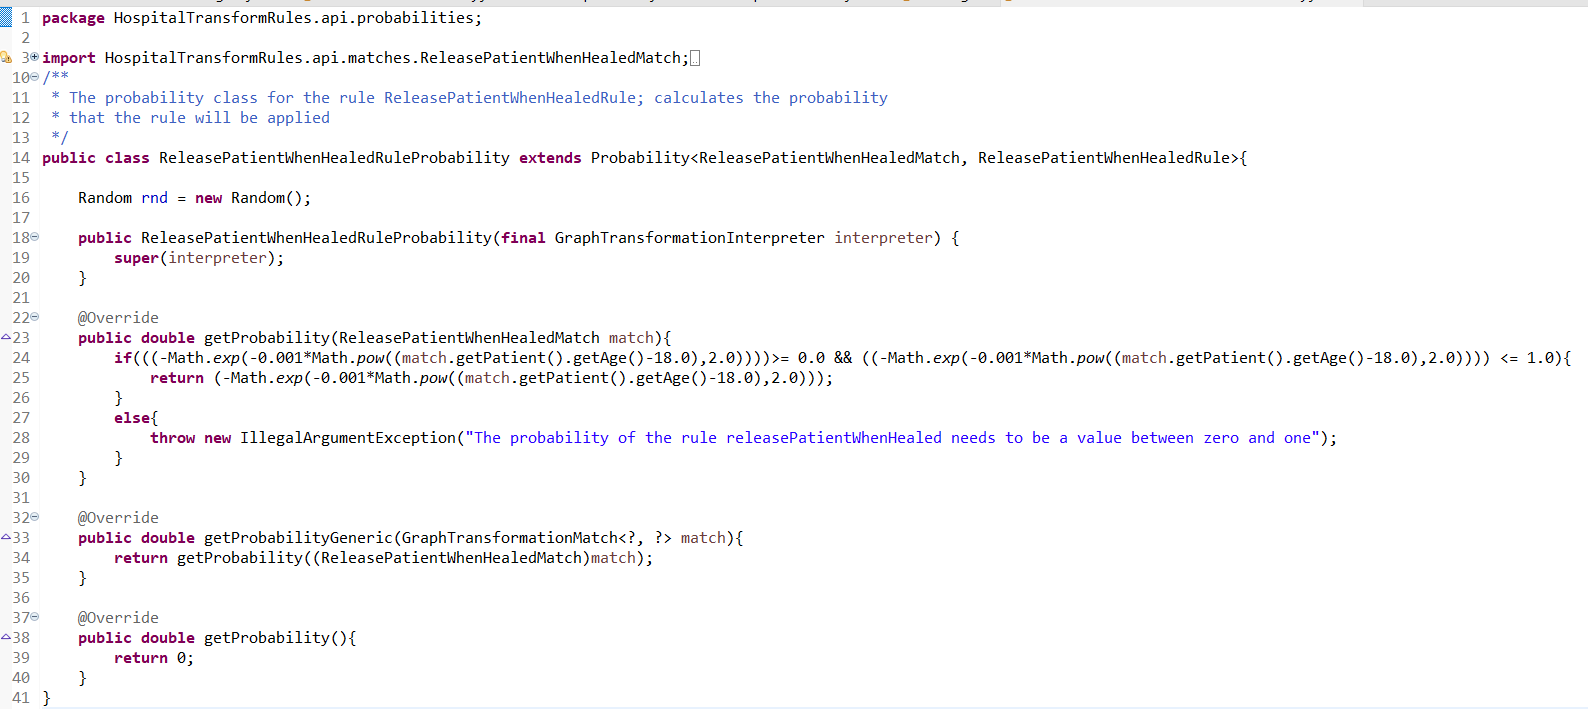
\includegraphics[scale=0.4]{pictures/probabilityClass.png}
    \caption{\centering{Probability Class}}
    \label{Probability Class in HospitalTransformRules.api.probabilities}
\end{figure}


All probability classes implement the \textbf{Probability interface}, which declares the methods \textsf{getProbability(M match)} and \textsf{getProbability()}. A generated probability class can only receive correct values when using the \textsf{getProbability(M match)} method since it needs the match to get the values of the parameters. When using the \textsf{getProbability()} method it will only return the value 0. The \textsf{StaticProbability} class can use both methods since it is not dependent on the match.\newline

\textbf{Error handling:}

When using parameterized probabilities, there is no need to check mathematical constraints in the condition definition. Constraints like division by zero will be automatically checked in the probability class, but the user is responsible for not violating any of them during execution of the actual code.\newline

\subsection{Stochastic functions}

Another way to describe the probability of a rule is with a stochastic function. With these functions, it is possible to define a randomly generated probability or to describe a probability defined as: $$P(X < k) $$

EMoflon supports the following stochastic functions: 

\begin{itemize}
    \item Normal distribution
    \item Uniform distribution
    \item Exponential distribution
\end{itemize}

Now we want to model the chance of recovery for a patient as a random probability $p$:
$$p \sim N(0,1)$$

{\setstretch{1.2}

1\hspace{0.5cm}\textcolor{Purple}{rule} releasePatientWhenHealed\{

\hspace{0.75cm}...

2\hspace{0.5cm} \}

3\hspace{0.5cm}\textcolor{Purple}{when} patientIsTreated @ N(0,1)\newline

}

The probability of applying thist rule will be calculated in eMoflon as p = \textsf{random.nextGaussian()}.

You can find the syntax for referencing the supported stochastic functions in the \textbf{appendix}.

\subsection{Number Generation}

Another useful feature of the stochastic distribution extension is the value generation function. With this feature, we can assign a randomly generated number of the specific distribution to an attribute. If the connect rule is expanded to designate a random flag to every connection, then the rule can be written as:\newline

{\setstretch{1.2}

1\hspace{0.5cm}\textcolor{Purple}{rule} createRandomPatient \{

2\hspace{1cm}\textcolor{LimeGreen}{++ patient: Patient}\{

3\hspace{1.5cm}.\textcolor{LimeGreen}{name} :=\textcolor{Blue}{"John Doe"}

4\hspace{1.5cm}.\textcolor{LimeGreen}{patientID} := \textcolor{Purple}{N}(100,15)

5\hspace{1.5cm}.\textcolor{LimeGreen}{level} :=\textcolor{Grey}{0}

6\hspace{1.5cm}.\textcolor{LimeGreen}{age} := +\textcolor{Purple}{U}(0,99)

7\hspace{1cm}\}

8\hspace{0.5cm}\} \newline

}

By assigning U(0,99) to the \textsf{age} attribute it will get a uniform distributed value between 0 and 99. The new extension also supports so-called range assignments to the stochastic functions. 

The user may define whether the generated value should be only positive, only negative, or both by adding a plus for positive values and adding a minus for negative values in front of the brackets of the distribution.\newline

The example above depicts an example with positive values. With this example rule, it is possible to generate a positive value for the bandwidth attribute that is distributed as $b \sim N(100,15)$:

\clearpage